\chapter{Internet de las Cosas en los museos} \label{cap:aproxTeoricas}

\addcontentsline{toc}{section}{Introducción}
        \textbf{\Large Introducción}\newline

        En este capítulo estaremos desglosando por secciones el análisis de la trascendencia de la aplicación del Internet de las Cosas en los museos en el ámbito internacional, así como la aplicación o no del mismo en los museos de nuestro país.
        Se hace un análisis de las arquitecturas propuestas por otros autores y la proposición de una para este trabajo.
        También se tienen en cuenta las variables que se miden en los museos para evitar el deterioro de los objetos y los posibles sensores a emplear para su control.
        Además, se analiza el tipo de comunicación más viable y efectiva según el emplazamiento, y finalmente los posibles sistemas de seguridad a instalar en la muestra.
    
    \section{Internet de las Cosas en museos internacionales}\label{sec:iotMundo}
        
        Hoy en día existen museos líderes en el tema de interacción con el público, como es el caso de los museos Digital Art Museum TeamLab Borderless de Japón y el Atelier de Lumieres de Francia. El primero de estos es un espacio que posee 10 mil metros cuadrados de proyección 3D, acompañados de juegos de luces y efectos especiales que llevan a los visitantes en medio de paisajes surrealistas. El segundo museo realiza macro proyecciones 360° de las obras más importantes de artistas como Van Gogh, Picasso, Chagall, entre otros. \cite{museoInterSalaLimpia}.\\

        En Maloka \footnote{Maloka es un museo interactivo que fomenta la pasión por el aprendizaje a partir de los lazos entre ciencia, tecnología, innovación y sociedad.}, Bogotá, las exhibiciones ponen a prueba los 5 sentidos de los visitantes, haciendo que tanto niños, como adultos disfruten un tiempo en familia repleto de nuevos conocimientos, incluyendo recorridos por salas interactivas y funciones de proyección de cine. \cite{maloka}.\\

        En el museo MUST en Lecce, Italia, se llevó a cabo la instalación de un dispositivo portátil que combina el reconocimiento de imágenes y las capacidades de localización para proporcionar automáticamente a los usuarios contenidos culturales relacionados con las obras de arte observadas. La información de localización se obtiene mediante una infraestructura Bluetooth Low Energy \footnote{Bluetooth Low Energy es una tecnología de red de área personal inalámbrica, diseñada y comercializada por Bluetooth SIG destinada a aplicaciones en el cuidado de la salud, fitness y beacons, seguridad y las industrias de entretenimiento en el hogar} instalada en el museo. Además, el sistema interactúa con la Nube para almacenar contenidos multimedia producidos por el usuario y compartir eventos generados por el entorno en sus redes sociales. Estos servicios interactúan con dispositivos físicos a través de un middleware multiprotocolo. \cite{museoItalia}.\\

        En el caso del Conjunto Monumental de San Domenico Maggiore, ubicado en Nápoles (Italia), dentro del mismo se han transformado más de 270 esculturas en obras de arte parlantes. Equipado con un tablero de sensores, cada objeto puede proponerse automáticamente a los visitantes, compartiendo su historia en diferentes modalidades e idiomas, lo que permite un proceso de disfrute novedoso durante una experiencia cultural. \cite{monumentoSanDomenico}.\\

        En la Universidad de El Cairo, Egipto, desarrollaron un sistema para la conservación de las piezas en los museos, un sistema que no solo mide los atributos del entorno, sino que también mantiene la seguridad de los artefactos al detectar cualquier prueba de contacto o movimiento. También controla la intensidad de la luz en función de la ocupación de la sección del museo. Una característica diferenciadora del sistema es el diseño de energía ultrabaja de su nodo sensor que conduce a una larga vida útil de hasta 50 días. \cite{ultraLowPowerConservacion}.\\
        
        Existen otros proyectos de utilización del Iot en museos, tal es el caso del proyecto propuesto en el III Congreso Internacional de Avances en Electricidad, Electrónica, Información, Comunicación y Bioinformática en el año 2017. El proyecto consiste en el montaje de un sistema que se basa en un dispositivo portátil que captura el movimiento del usuario, realiza el algoritmo de sustracción de fondo para realizar el procesamiento de imágenes y obtiene la información de localización de un Bluetooth Low Energy (BLE).\cite{proyectoIotdispositivoPortatil}. En agosto del 2019, entre la Escuela de Ingeniería Electrónica, Universidad de Jiujiang y la Escuela de Ciencias de la Computación, Universidad de Wuhan, ambas de China elaboraron un artículo donde propusieron un esquema antirrobo para museos basado en la tecnología Internet of Things (IoT), que identifica si las reliquias culturales están dentro del rango seguro a través de lectores/escritores RFID (identificación por radiofrecuencia del inglés Radio Frequency Identification) pasivos. \cite{chinaSistemaSeguridadRFID}.\\

        La siguiente tabla resume lo anterior expuesto.

        \begin{table}[h]
            \begin{tabular}{|l|l|l|}
                \hline
                \rowcolor[HTML]{9698ED} 
                Aplicación IoT                                                                                                                                                        & Lugar                                                                                            & Referencia                                                                                       \\ \hline
                \begin{tabular}[c]{@{}l@{}}Proyección 3D y efectos\\ especiales\end{tabular}                                                                                          & \begin{tabular}[c]{@{}l@{}}Digital Art Museum TeamLab \\ Borderless de Japón\end{tabular}        & \begin{tabular}[c]{@{}l@{}}(Corzo Vargas\\ y cols., 2019)\end{tabular}                           \\ \hline
                \begin{tabular}[c]{@{}l@{}}Proyecciones 360° de obras\\ importantes de artistas.\end{tabular}                                                                         & \begin{tabular}[c]{@{}l@{}}Atelier de Lumieres de \\ Francia.\end{tabular}                       & \begin{tabular}[c]{@{}l@{}}(Corzo Vargas\\ y cols., 2019).\end{tabular}                          \\ \hline
                \begin{tabular}[c]{@{}l@{}}Recorridos por salas \\ interactivas y proyecciones\\ de cine.\end{tabular}                                                                & Maloka, Bogotá.                                                                                  & \begin{tabular}[c]{@{}l@{}}(Pinzón Ortega, \\ Franco Avellaneda, \\ y Falla, 2015).\end{tabular} \\ \hline
                \begin{tabular}[c]{@{}l@{}}Reconocimiento de\\ imágenes y capacidades de\\ localización proporcionando\\ contenido cultural.\end{tabular}                             & Museo MUST en Lecce, Italia.                                                                     & (Alletto y cols., 2016).                                                                         \\ \hline
                \begin{tabular}[c]{@{}l@{}}Obras de arte parlantes\\ equipadas con tableros de\\ sensores. Cada obra de arte\\ comparte su historia.\end{tabular}                     & \begin{tabular}[c]{@{}l@{}}Conjunto Monumental de San \\ Domenico Maggiore, Italia.\end{tabular} & \begin{tabular}[c]{@{}l@{}}(Chianese,\\ Piccialli, y Jung, 2016).\end{tabular}                   \\ \hline
                \begin{tabular}[c]{@{}l@{}}Sistema para la conservación\\de las piezas en los museos\\en base a pruebas\\de contacto o movimiento,\\intensidad de la luz.\end{tabular}&Universidad de El Cairo, Egipto                                                                   & \begin{tabular}[c]{@{}l@{}}(Al-Habal\\y Khattab, 2019).\end{tabular}                             \\ \hline
            \end{tabular}
        \end{table}

        \vspace{2cm}

        \begin{table}[h]
            \begin{tabular}{|lll|}
                \hline
                \multicolumn{3}{|c|}{Continuación Tabla \ref{tab: iotInternacional}}                                                                                                                                                                                                                                                                                                                                                                                    \\ \hline
                \multicolumn{3}{|c|}{Proyectos}                                                                                                                                                                                                                                                                                                                                                                                                 \\ \hline
                \multicolumn{1}{|l|}{\begin{tabular}[c]{@{}l@{}}Captura el movimiento del\\ usuario, procesamiento de\\ imágenes.\end{tabular}} & \multicolumn{1}{l|}{\begin{tabular}[c]{@{}l@{}}III Congreso Internacional de\\ Avances en Electricidad,\\ Electrónica, Información,\\ Comunicación y\\ Bioinformática en el año 2017\end{tabular}}                & \begin{tabular}[c]{@{}l@{}}(Sornalatha y \\ Kavitha, 2017).\end{tabular}  \\ \hline
                \multicolumn{1}{|l|}{\begin{tabular}[c]{@{}l@{}}Propuesta de esquema\\ antirrobo para museos\\ basados en IoT.\end{tabular}}    & \multicolumn{1}{l|}{\begin{tabular}[c]{@{}l@{}}Escuela de Ingeniería Electrónica,\\ Universidad de Jiujiang\\ y la Escuela de Ciencias de\\ la Computación, Universidad de\\ Wuhan, ambas de China.\end{tabular}} & \begin{tabular}[c]{@{}l@{}}(Liu, Wang, Qi, y Yang, \\ 2019).\end{tabular} \\ \hline
                \end{tabular}
            \caption{IoT Internacional}
            \subcaption*{Fuente: Elaboración propia}
            \label{tab: iotInternacional}
        \end{table}
                
        Como podemos observar en la tabla \ref{tab: iotInternacional} existen disímiles ejemplos de aplicación del Internet de las Cosas a nivel internacional; de ahí que haremos énfasis en la aplicación de sistemas de conservación de las piezas en los museos tomando como referencia los ejemplos anteriormente expuestos.

    \section{Internet de las Cosas en Cuba}\label{sec:iotCuba} 
        En Cuba existen escasos ejemplos de la aplicación del Internet de las Cosas en los museos, no obstante, dentro de esos pocos se encuentra el Palacio del Segundo Cabo.\\
        
        Desde 2012 se venía proyectando una sala dedicada al libro cubano, con la cooperación de la Unión Europea y la Unesco. \cite{oficinaHistoriadorRescatepatrimonio}. Gracias a este Rescate Patrimonial y Desarrollo Cultural en La Habana, se propició la restauración del mismo para la creación del Centro. Esta iniciativa de cooperación internacional fue desarrollada por la Oficina del Historiador de la Ciudad de La Habana, con apoyo de la Unión Europea y de la Organización de Naciones Unidas para la Educación, la Ciencia y la Cultura (UNESCO). \cite{potencialidadProyectoMuseologico}.\\
        
        El Centro cuenta con una sala monográfica que propone un audiovisual realizado por autores cubanos donde se relata la historia del inmueble donde está ubicada la institución. Además, de una sala introductoria que refleja la visión que se tenía antes del encuentro de las dos culturas con la llegada de Cristóbal Colón. Este relata en paralelo la historia de Cuba y de Europa interrelacionadas en un ambiente inmersivo y por fuera se puede recorrer desde la visión de las artes plásticas europeas y cubanas. Siempre están acompañados de cuatro audiovisuales que recorren líneas independientes como la historia de la esclavitud, la ciencia, los servicios públicos y la economía.\\
        
        Adosada a esta sala se encuentra la de llegada y migraciones donde en un espacio se reproduce una parte de un galeón, atractivo para el público pues puede sentirse una ligera «brisa de mar», una corriente de aire situada en la parte posterior del barco. Esto se complementa con dos pantallas y proyectores que permiten la visualización de un audiovisual que también habla de las llegadas de los aborígenes, los conquistadores; la migración forzada de los africanos y así sucesivamente con las diferentes olas migratorias que han formado la actual característica mestiza de nuestra identidad y nación.\\
        
        La Sala de Viajeros se soporta en un software que despliega una galería de imágenes ya sea de cubanos relevantes de visita por Europa o de europeos de visita en Cuba. Mediante el uso de pantallas táctiles, el visitante puede interactuar con las imágenes de las personalidades, leer una síntesis biográfica e incluso escuchar muestras de audio.
    
        
    \section{Arquitectura IoT}\label{sec:arquitecturas}

    Lo primero que debemos saber sobre la arquitectura de IoT, es que no existe una única definición universalmente adoptada. Diferentes propuestas han surgido durante su desarrollo entre las que podemos encontrar: la arquitectura de 3 capas, la arquitectura de 5 capas, la arquitectura de nube, la arquitectura de niebla y la arquitectura de computación de Borde entre muchas otras \cite{arquitecturaIEEE}.\\\\\\\\\\\\

    En la figura \ref{imag:comparacionArquitecturas} se observa una comparación entre las arquitecturas de 3 capas, 5 capas y la arquitectura de nube.

    \begin{figure}[h]
        \centering
        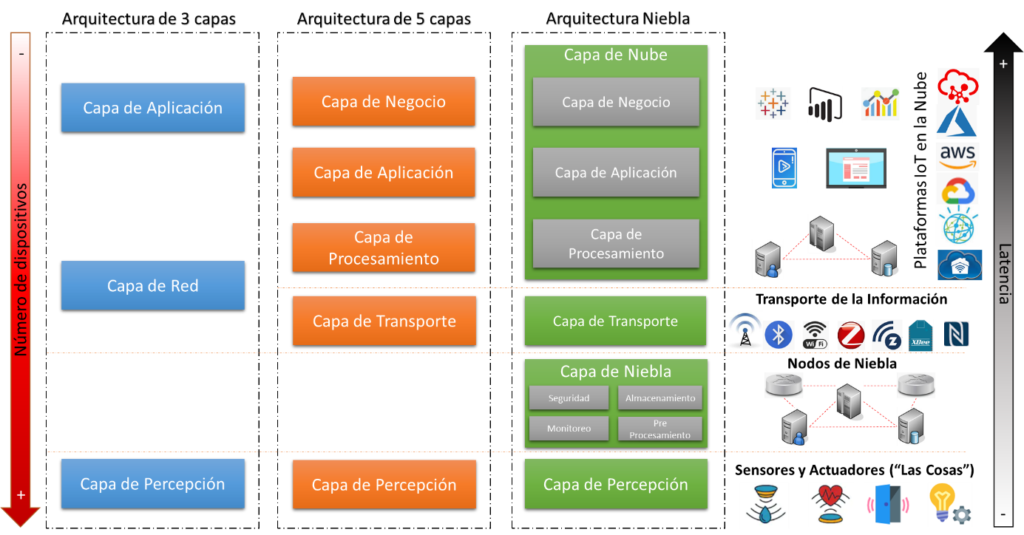
\includegraphics[width=10cm, height=6cm]{imagenes/Comparacion-arquitecturas-1024x535}
        \caption{Comparación arquitecturas}
            \subcaption*{Fuente: \cite{arquitecturaPaginaLuisGarcia}}
        \label{imag:comparacionArquitecturas}
    \end{figure}

    Según \cite{capasIoTciberseguridad}, la mayoría de estas arquitecturas de IoT se basan en fundamentos básicos:
    \begin{itemize}
        \item Dispositivos más inteligentes en una forma diferente.
        \item Red y puerta de enlace que permite que los dispositivos formen parte del IoT.
        \item Middleware que incluye espacios de almacenamiento de datos y avances en las capacidades de predicción.
        \item Aplicaciones de usuario final.
    \end{itemize}

    Las propuestas de arquitecturas pueden variar de autor en autor, en dependencia de la estructura del sistema IoT propuesto. Dichas arquitecturas son desarrolladas por capas en las que se agrupan los objetos, dispositivos, sensores, actuadores, etcétera.

    \subsection{Principales capas de la arquitectura del IoT}

    Según  \cite{internetOfThingsStateOfTheArt}, dentro de las capas más importantes del IoT podemos encontrar:

    \begin{itemize}
        \item \textit{La capa de percepción} (Objetos/ Dispositivos/ SensorActuador/ WSN/ Edge Computing/ Sensado), digitaliza y transfiere datos a la capa de red, a través de canales seguros. Se localizan los objetos físicos, dispositivos sensores y actuadores utilizados para recopilar información del contexto.
        \item \textit{La capa de acceso} (Adaptación/ Observador), comprueba la información que recibe de la capa de percepción, si está protegida o no contra intrusos y virus. Si hay algún ataque, no pasa los datos a la siguiente capa. También verifica la identidad y autenticación de los objetos.
        \item \textit{La capa de Red} (Abstracción de Objetos/ Transporte/ Fog computing), transporta y transmite los datos, recopilados de la capa de percepción, hacia la cloud. Se localizan componentes de red (switch, router, Gateway, etc.), medios de comunicación y protocolos. También es responsable de aspectos de seguridad y el control de ataques.
        \item \textit{La Capa Aplicación / Cloud Computing (CC)} en modelos de más de tres capas, puede dividirse en:
            \begin{itemize}
                \item \textit{Capa de procesamiento y almacenamiento, Soporte, o Middleware}. Permite a los programadores de aplicaciones IoT trabajar con objetos heterogéneos sin tener en cuenta una plataforma de hardware específica. Se encarga de integrar, almacenar, procesar y analizar datos, tomar decisiones y ofrecer servicios de protocolos de conexión de red.
                \item \textit{La capa de aplicación}, define los servicios y funciones que proporciona la aplicación IoT implementada (hogar inteligente, ciudad inteligente, salud inteligente, etc.) a los clientes. Los servicios pueden variar para cada aplicación y depende de la información que se recopilan de los sensores. También se consideran aspectos de seguridad.
                \item \textit{La capa empresarial}, tiene la responsabilidad de administrar y controlar el comportamiento de las aplicaciones, modelos de negocios y ganancias de IoT. También tiene la capacidad de determinar cómo se puede crear, almacenar y cambiar la información. Administra la privacidad del usuario y evita vulnerabilidades.\\\\\\\\
            \end{itemize} 
    \end{itemize}

    \subsection{Propuesta de la Arquitectura IoT del Sistema}

    En base de los esquemas de arquitecturas propuestas, definimos el uso de la arquitectura del proyecto la cual se cimienta en la estructura de cuatro capas, considerando las diferentes capas que son: La capa de percepción cuya función es la obtención de variables asociadas a la conservación de las piezas en la muestra, la capa de transporte con el propósito de transportar la data recopilada por los sensores para su posterior procesamiento y análisis, la capa de procesamiento que genera predicciones y recomendaciones expuesta a cambios constantes de los valores que se reciben desde el comienzo del ciclo en la etapa de percepción y, la capa de aplicación, la cual permite a los usuarios finales visualizar en una interfaz y mediante el empleo de la RA (Realidad Aumentada), los datos y predicciones en dependencia de la información recopilada.\\

    \begin{figure}[h]
        \centering
        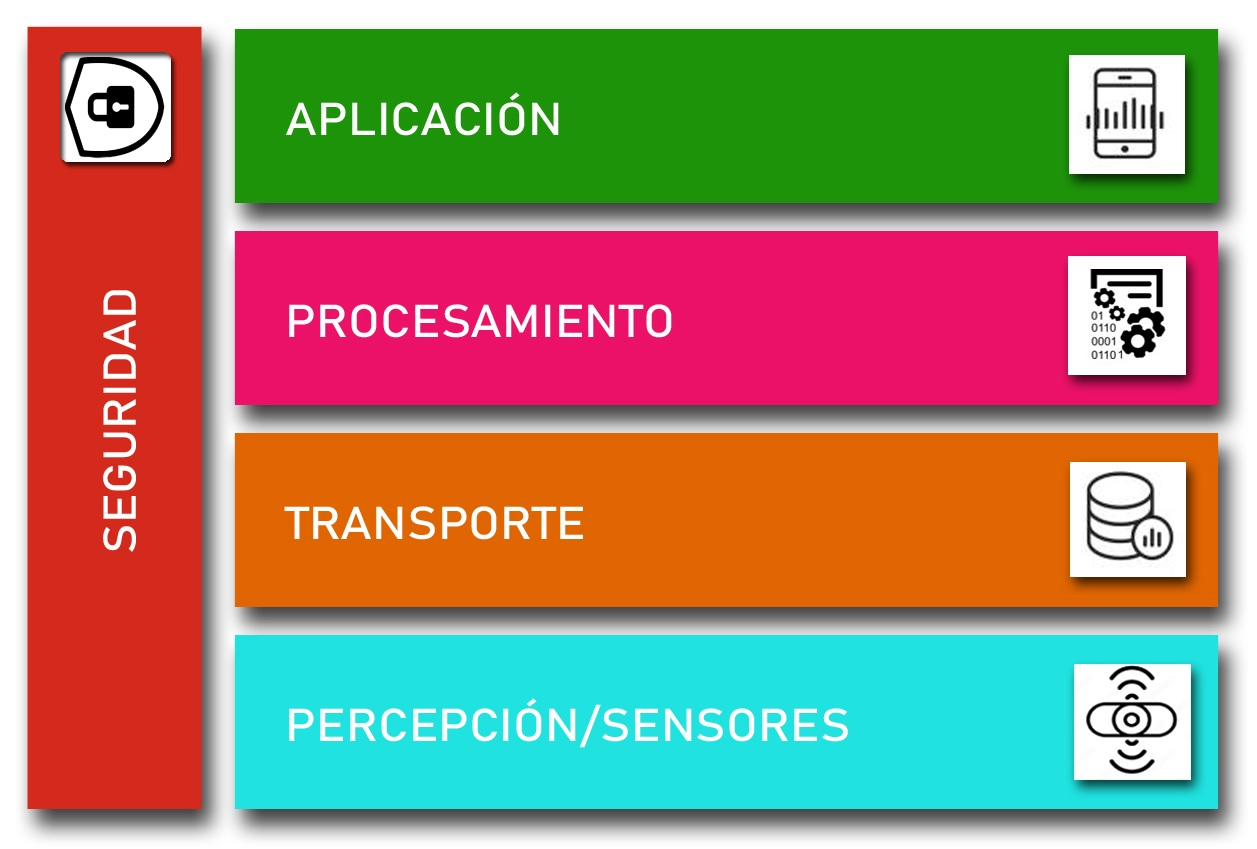
\includegraphics[width=10cm, height=6cm]{imagenes/myArquitecture0.jpg}
        \caption{Vista funcional de la arquitectura}
            \subcaption*{Fuente: Elaboración propia}
        \label{imag:arquitecturaPropuesta}
    \end{figure}

    \subsection{Capa de percepción}\label{subsec:capa_percepcion}
    En esta capa de percepción se encuentran los sensores que, de manera general recopilarán los datos para luego ser enviados a su procesamiento. La muestra Prat está distribuida de tal modo que las piezas están ubicadas en tres salas expositivas. Enumerándolas: sala 1, sala 2 y sala 3.\\\\

    La sala 1 (Exposición permanente) está caracterizada por la presencia de varios objetos distribuidos en vitrinas, sobre mesas, colgados, en estantes empotrados en la pared, o en pedestales. Se observan varios objetos de cerámica, marfil, metal, piedra, madera etcétera.\newline
    [Imagen de la sala 1]\newline
    En la sala 2 solamente se encuentran tres pinturas pertenecientes a la colección, éstas poseen también condiciones de deterioro notables por el efecto de la humedad y del nivel de luz dentro del local. La humedad provoca la aparición de hongos en el lienzo deteriorándolo y dañando también el color.\newline
    [Imagen de uno de los cuadros donde se sea el hongo] (Nombre || Fuente).\newline
    Dentro de la sala 3 se localizan también varios objetos ubicados en pedestales mostrando colecciones de medallas y objetos personales del mismo Prat Puig y, además, vitrinas donde se hallan, principalmente, objetos de cerámica como platos, jarrones y cántaros.\newline
    [Imagen sala 3]\newline
    En la siguiente tabla se relaciona el valor cuantitativo de las principales formas en las que se exponen las piezas dentro de estas salas:\newline


        \begin{table}[h]
            \begin{center}
            \begin{tabular}{|l|r|}
            \hline
            \rowcolor[HTML]{9698ED} 
            \multicolumn{1}{|r|}{\cellcolor[HTML]{9698ED}Ubicación} & Cantidad \\ \hline
            Vitrinas                                                & 12       \\ \hline
            Mesas                                                   & 2        \\ \hline
            Estantes                                                & 1        \\ \hline
            Colgados                                                & 23       \\ \hline
            Pedestales                                              & 3        \\ \hline
            \end{tabular}
            \caption{Ubicación piezas}
            \subsection*{Fuente: Elaboración propia}
            \label{tab:valor_cuantitativo}
        \end{center}
        \end{table}

    Según la tabla \ref{tab:valor_cuantitativo}, varios objetos están dispuestos dentro de vitrinas por lo que la condición ambiental en estas es diferente a la condición ambiental del local, de ahí la necesidad de incorporar nodos de tal manera que se tomen los datos dentro de estas vitrinas por separado y además un nodo general para el caso de las piezas que se encuentran fuera.\\\\

    \textbf{Nodos}\\
    Los nodos que, de manera general, recopilarán los datos de cada sala, estarán compuestos por los sensores que permitan medir los valores de temperatura, humedad, polución, CO2, vibraciones y luminosidad mientras que, en el caso de los nodos dentro de las vitrinas, se tiene en cuenta las condiciones del microclima y el material de los objetos.\\

    En la tabla que se muestra a continuación se hace una analogía de las características de los nodos que estarán presentes:\\

    \begin{table}[h]
        \centering
        \begin{tabular}{|l|c|l|c|}
        \hline
        \rowcolor[HTML]{9698ED} 
        \multicolumn{1}{|r|}{\cellcolor[HTML]{9698ED}Nodo} & \multicolumn{1}{r|}{\cellcolor[HTML]{9698ED}Cantidad}                       & Meterial objetos                                                                            & \multicolumn{1}{l|}{\cellcolor[HTML]{9698ED}Variable a medir}                                                                    \\ \hline
        1                                                  & \begin{tabular}[c]{@{}c@{}}General\\ Sala 1\end{tabular}                    & \multicolumn{1}{c|}{porcelana, barro, marfil}                                               & \begin{tabular}[c]{@{}c@{}}temperatura, humedad,\\ polución, luminosidad,\\ CO2, vibraciones, salitre,\\ xilófagos\end{tabular}  \\ \hline
        2                                                  &                                                                             & bronce, barro, arcilla, piedra                                                              &                                                                                                                                  \\ \cline{1-1} \cline{3-3}
        3                                                  &                                                                             & colección numismática                                                                       &                                                                                                                                  \\ \cline{1-1} \cline{3-3}
        4                                                  &                                                                             & cerámica, madera, barro, bronce                                                             &                                                                                                                                  \\ \cline{1-1} \cline{3-3}
        5                                                  &                                                                             & \begin{tabular}[c]{@{}l@{}}madera, bronce, plata, cerámica,\\ porcelana, cuero\end{tabular} &                                                                                                                                  \\ \cline{1-1} \cline{3-3}
        6                                                  &                                                                             & barro, cerámica, plata                                                                      &                                                                                                                                  \\ \cline{1-1} \cline{3-3}
        7                                                  &                                                                             & bronce, marfil, madera                                                                      &                                                                                                                                  \\ \cline{1-1} \cline{3-3}
        8                                                  & \multirow{-7}{*}{\begin{tabular}[c]{@{}c@{}}Vitrinas\\ Sala 1\end{tabular}} & porcelana, barro policromado                                                                & \multirow{-7}{*}{\begin{tabular}[c]{@{}c@{}}temperatura, humedad,\\ luminosidad, vibraciones.\end{tabular}}                      \\ \hline
        9                                                  & \begin{tabular}[c]{@{}c@{}}General\\ Sala 2\end{tabular}                    & tela, madera                                                                                & \begin{tabular}[c]{@{}c@{}}temperatura, humedad,\\ polución, luminosidad,\\ CO2, salitre, xilófagos.\end{tabular}                \\ \hline
        10                                                 & \begin{tabular}[c]{@{}c@{}}General\\ Sala 3\end{tabular}                    & metal, plástico, tela, cuero, madera                                                        & \begin{tabular}[c]{@{}c@{}}temperatura, humedad,\\ polución, luminosidad,\\ CO2, vibraciones, salitre,\\ xilófagos.\end{tabular} \\ \hline
        11                                                 &                                                                             &                                                                                             &                                                                                                                                  \\ \cline{1-1}
        12                                                 &                                                                             &                                                                                             &                                                                                                                                  \\ \cline{1-1}
        13                                                 &                                                                             &                                                                                             &                                                                                                                                  \\ \cline{1-1}
        14                                                 & \multirow{-4}{*}{\begin{tabular}[c]{@{}c@{}}Vitrinas\\ Sala 3\end{tabular}} & \multirow{-4}{*}{cerámica (barro)}                                                          & \multirow{-4}{*}{\begin{tabular}[c]{@{}c@{}}temperatura, humedad,\\ luminosidad, vibraciones.\end{tabular}}                      \\ \hline
        \end{tabular}
        \caption{Correlación de los nodos}
        \subcaption*{Fuente: Elaboración propia}
        \label{tab:correlacion_nodos}
    \end{table}

    Estos nodos estarán constituidos por un controlador, una serie de sensores y su correspondiente alimentación.\\\\

    \textbf{Microcontrolador}

    Dentro de la familia de los ESP (significado) se encuentra el NodeMcu (Imagen \ref{imag:nodemcu}). Este microcontrolador (referenciar figura) será el encargado de recibir los datos de los sensores y organizarlos en función de su continua transmisión hacia el concentrador.\\

    \begin{figure}[h]
        \centering
        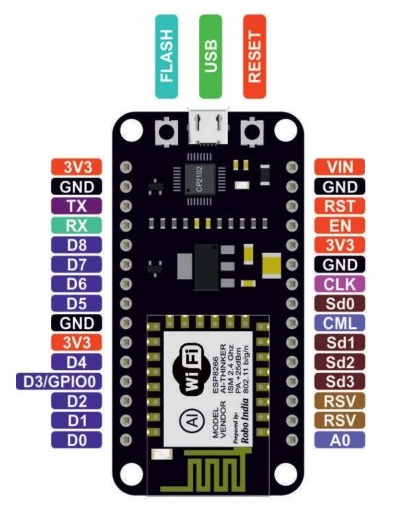
\includegraphics[width=5cm, height=6cm]{imagenes/nodemcu0.jpg}
        \caption{Esquemático NodeMcu Vendor}
        \label{imag:nodemcu}
    \end{figure}
    
    
    NodeMCU es una pequeña placa Wifi compatible con Arduino, lista para usar en cualquier proyecto IoT. Está montada alrededor del microcontrolador ESP8266 y expone todos sus pines en los laterales. Además, ofrece más ventajas como la incorporación de un regulador de tensión integrado, así como un puerto USB de programación. Se puede programar con LUA o mediante el IDE de Arduino.\\

    Dispone de una extensa comunidad y documentación que permitirá conectar el proyecto mediante conexión Wifi.\\

    \textbf{Características}
    \begin{itemize}
        \item Procesador: ESP8266 a 80MHz (3.3V) (ESP-12E).
        \item 4MB de memoria FLASH (32 MBit).
        \item WiFi 802.11 b/g/n.
        \item Regulador 3.3V integrado (500mA).
        \item Conversor USB-Serial CH340G / CH340G.
        \item Función Auto-reset.
        \item 9 pines GPIO con I2C y SPI.
        \item 1 entrada analógica (1.0V max).
        \item 4 agujeros de montaje (3mm).
        \item Pulsador de RESET.
        \item Entrada alimentación externa VIN (20V max).\\
    \end{itemize}

    \textbf{Sensores}\\
    En el caso de los sensores, la siguiente tabla relaciona el sensor a emplear según la variable a controlar.

    \begin{table}[h]
        \centering
        \begin{tabular}{|c|c|l|}
        \hline
        \rowcolor[HTML]{9698ED} 
        \multicolumn{1}{|l|}{\cellcolor[HTML]{9698ED}Variable a controlar} & Sensor     & \multicolumn{1}{c|}{\cellcolor[HTML]{9698ED}Descripción}                                                                                    \\ \hline
        Temperatura                                                        & DHT22      & \begin{tabular}[c]{@{}l@{}}Rango Temperatura: De - 40 a 80°C\\ Voltaje de alimentación: De 3V a 6V\\ Corriente: De 1mA a 1.5mA\end{tabular} \\ \hline
        Humedad                                                            & DHT22      & \begin{tabular}[c]{@{}l@{}}Rango Humedad: De 0 a 100\%r\\ Voltaje de alimentación: De 3V a 6V\\ Corriente: De 1mA a 1.5mA\end{tabular}      \\ \hline
        Polución                                                           & SDS011     & \begin{tabular}[c]{@{}l@{}}Rango: De 0.0 a 999.9ugm3\\ Voltaje de alimentación: 5V\\ Corriente: 100mA máxima\end{tabular}                   \\ \hline
        Luminosidad                                                        & BH1750     & \begin{tabular}[c]{@{}l@{}}Rango: De 1 a 65535Lx\\ Voltaje de alimentación: 5V\\ Corriente: 10mA\end{tabular}                               \\ \hline
        CO2                                                                & MH-Z19C    & \begin{tabular}[c]{@{}l@{}}Rango: De 400ppm a 5000ppm\\ Voltaje de alimentación:5V\\ Corriente: menor a los 40mA\end{tabular}               \\ \hline
        Vibraciones                                                        & M0168(OEM) & \begin{tabular}[c]{@{}l@{}}Salida analógica\\ Voltaje de alimentación: De 3.3V a 5V\\ Corriente: 10mA\end{tabular}                          \\ \hline
        Salitre                                                            & -          & Obtenida por predicciones.                                                                                                                  \\ \hline
        Xilófagos                                                          & -          & Obtenida por predicciones.                                                                                                                  \\ \hline
        \end{tabular}
        \caption{Relación sensores}
        \subcaption*{Fuente: Elaboración propia}
        \label{tab:relacion_sensores}
    \end{table}

    La medida del nivel de salitre, como se muestra en la tabla (ref), es obtenida mediante el análisis del nivel de humedad presente en los locales de la muestra.\\
    …

    En el caso del control de la aparición de los xilófagos, esta es obtenida a partir del análisis de las condiciones óptimas para la aparición de los mismos. Normalmente estos aparecen cuando la madera se encuentra con un porcentaje de humedad excesivo (por encima del 20 por ciento. Según \cite{monitoringMoisture} el porcentaje de humedad óptimo para que crezcan los xilófagos está entre el 25 y el 55 por ciento mientras que \cite{woodPreservation} plantea que, el rango de humedad idónea puede estar entre el 35 y el 50 por ciento. Tomando estos porcentajes de humedad idóneos para la aparición de los xilófagos, se establece como valor máximo de humedad un 20 por ciento.\\

    La temperatura también influye en la aparición de los xilófagos a tal nivel …\\


    \textbf{Alimentación} 


    \subsection{Capa de transporte}\label{subsec:capa_transporte}
    Entre las tres salas que componen la muestra existes una separación considerable por ello la necesidad de incorporar una comunicación inalámbrica.

    \subsection{Capa de procesamiento}\label{subsec:capa_procesamiento}
    El procesamiento de toda la data ...
    
    \subsection{Capa de aplicación}\label{subsec:capa_aplicacion}
    Pantalla TFT y Realidad Aumentada ...\newline


    \begin{figure}[h]
        \centering
        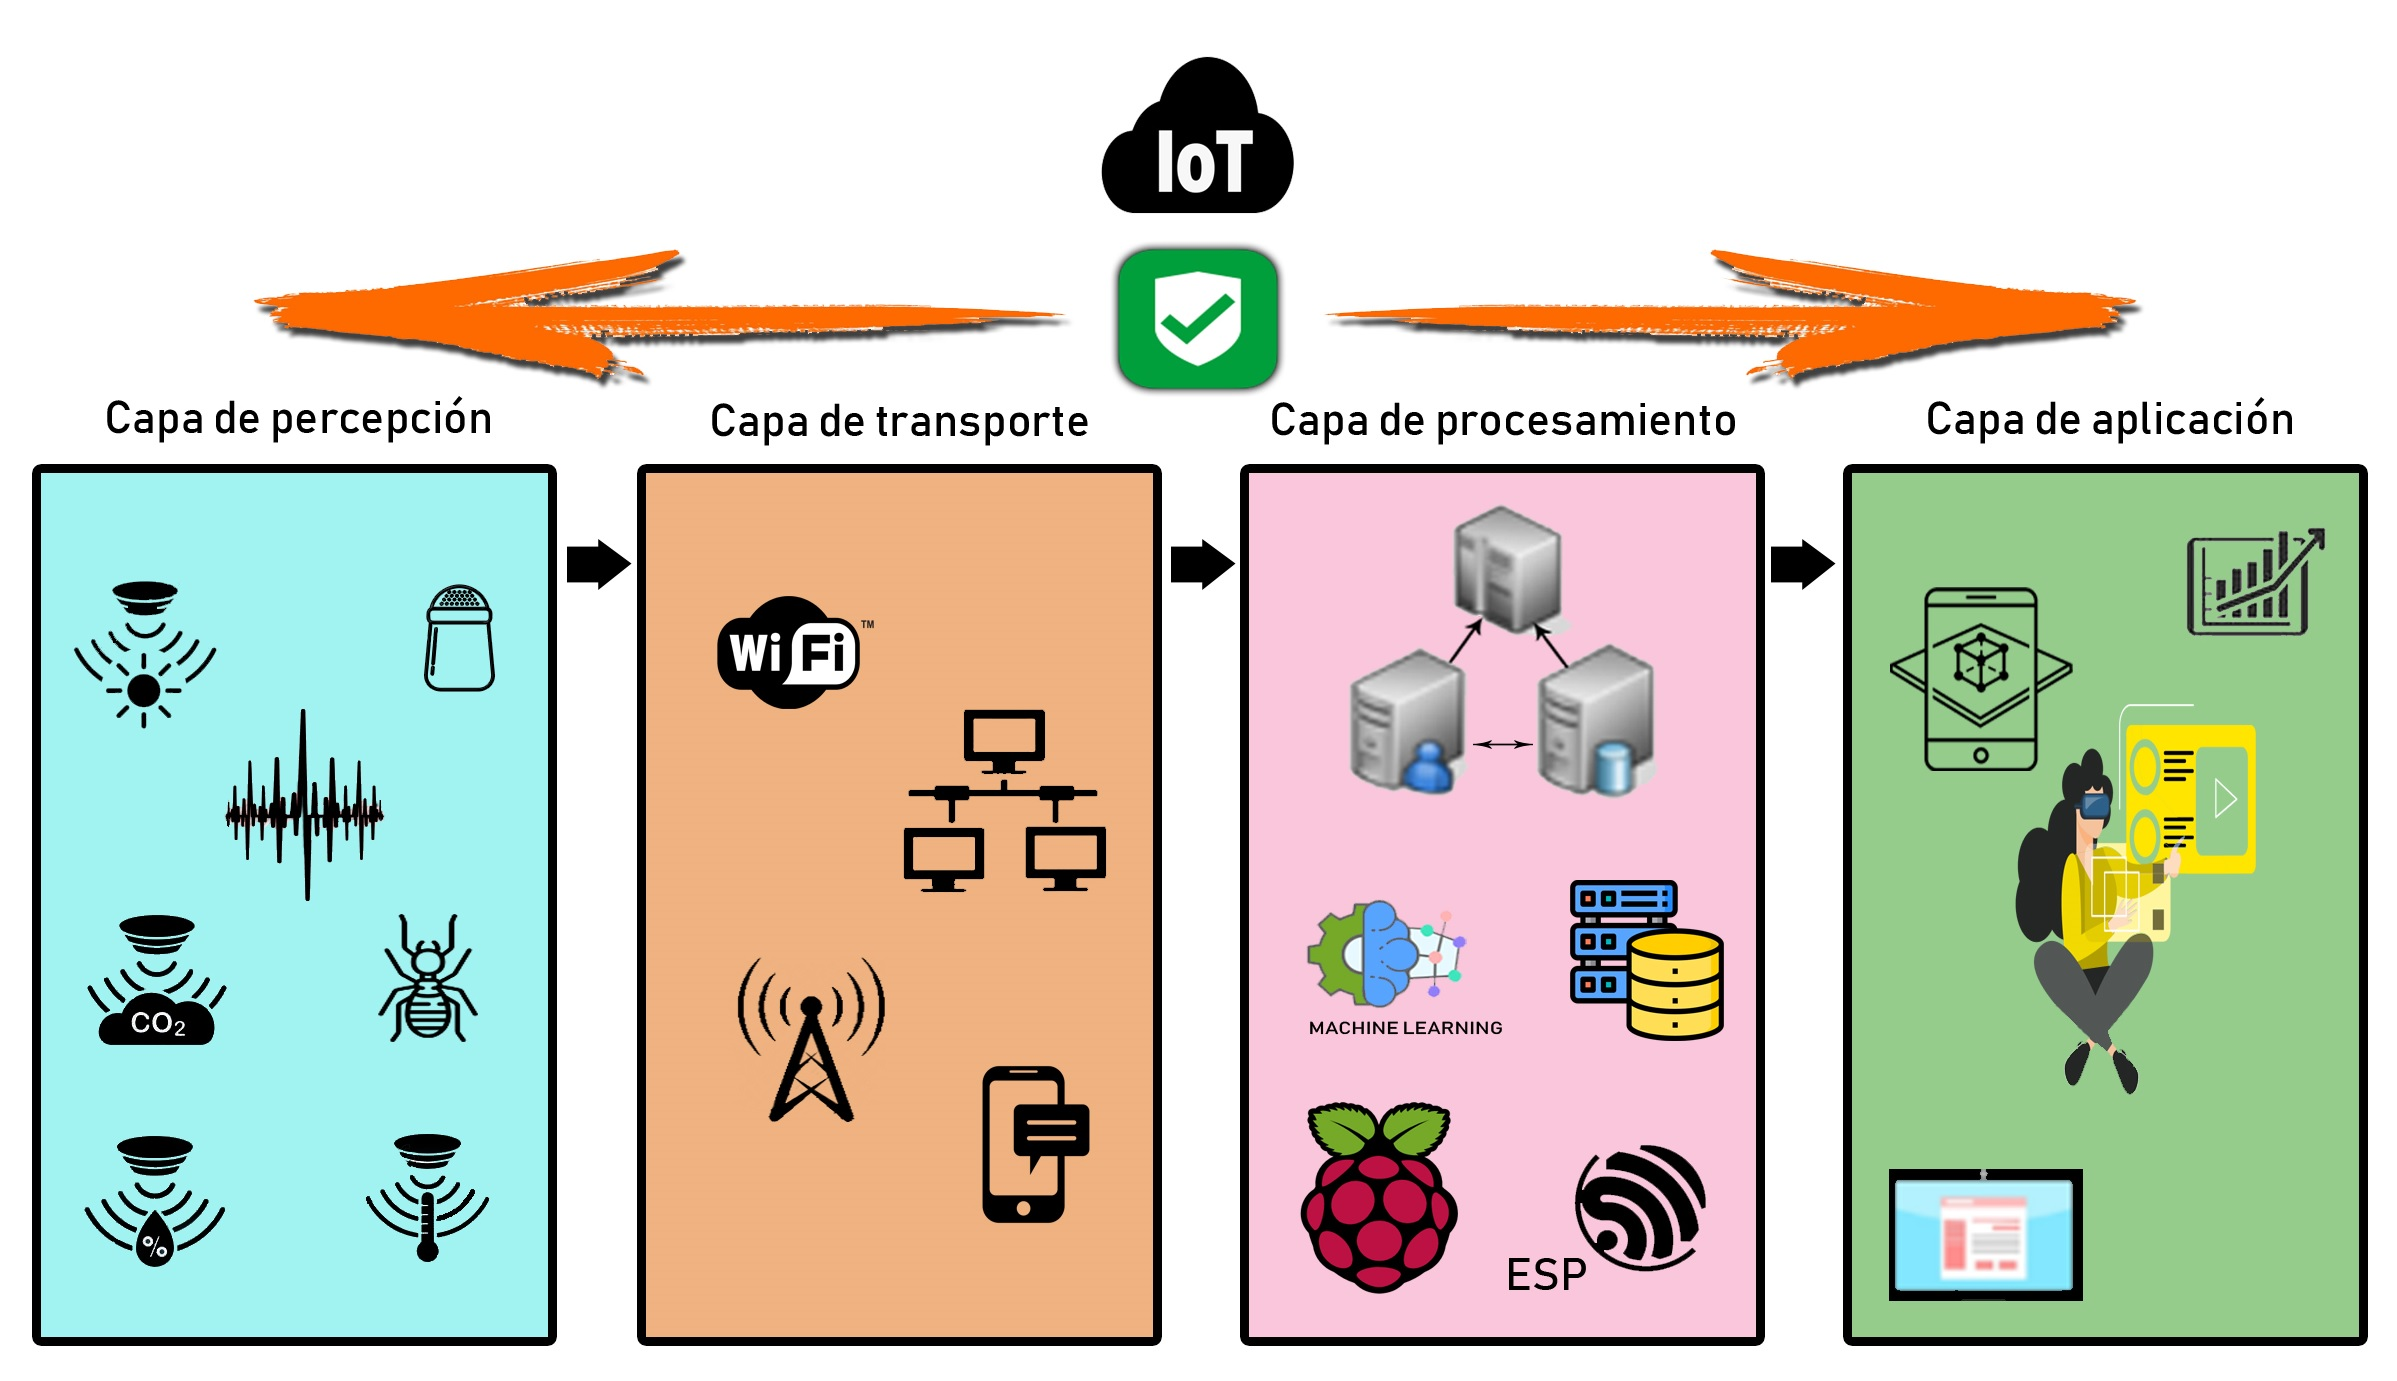
\includegraphics[width=10cm, height=6cm]{imagenes/myArquitecture.jpg}
        \caption{Vista de implementación}
            \subcaption*{Fuente: Elaboración propia}
        \label{imag:descripcionArquitectura}
    \end{figure}

    ...\newline

    Así, esta arquitectura pretende servir de referencia para la implementación de servicios basados en IoT en el área de conservación de las piezas en los museos o instituciones con vista al desarrollo de entornos inteligentes.\\

    %\section{Análisis de variables y sensores}\label{sec: analisisVariables}

    %\section{Sistema de comunicación}\label{sec: sistemaComunicación}

    \section{Sistema de seguridad}\label{sec: sistemaSeguridad}
    Sensores PIR y ESP32-CAM.\\

    \addcontentsline{toc}{section}{Conclusiones}
    \textbf{\Large Conclusiones}\newline